\documentclass[10pt]{article}
\usepackage[margin=0.45in]{geometry}
\usepackage{multicol}
\usepackage{amsmath,amssymb,mathtools}
\usepackage[most]{tcolorbox}
\usepackage{graphicx}
\usepackage{tikz}
\usepackage{enumitem}
\usepackage[table]{xcolor}
\usepackage{booktabs}
\usepackage{array}
\usepackage[hidelinks]{hyperref}
\usetikzlibrary{arrows.meta,calc,positioning,shapes.geometric,fit,backgrounds}
\setlength{\parindent}{0pt}
\setlength{\parskip}{2pt}

% ---------- colours ----------
\definecolor{bluepale}{RGB}{220,232,255}
\definecolor{greenpale}{RGB}{220,245,220}
\definecolor{orangepale}{RGB}{255,235,210}
\definecolor{redpale}{RGB}{255,220,220}
\definecolor{purplepale}{RGB}{240,225,255}
\definecolor{graypale}{RGB}{240,240,240}
\definecolor{greenlt}{RGB}{210,240,210}
\definecolor{accent}{RGB}{0,70,160}
\definecolor{accentg}{RGB}{0,120,60}

% ---------- tcolorbox styles ----------
\tcbset{
  intubox/.style={colback=bluepale,colframe=accent,
    fonttitle=\bfseries\footnotesize,title=#1,
    left=2pt,right=2pt,top=2pt,bottom=2pt,boxsep=1pt},
  formulabox/.style={colback=greenpale,colframe=accentg,
    fonttitle=\bfseries\footnotesize,title=#1,
    left=2pt,right=2pt,top=2pt,bottom=2pt,boxsep=1pt},
  warnbox/.style={colback=redpale,colframe=red!70!black,
    fonttitle=\bfseries\footnotesize,title=#1,
    left=2pt,right=2pt,top=2pt,bottom=2pt,boxsep=1pt},
  analogybox/.style={colback=orangepale,colframe=orange!70!black,
    fonttitle=\bfseries\footnotesize,title=#1,
    left=2pt,right=2pt,top=2pt,bottom=2pt,boxsep=1pt},
  summarybox/.style={colback=purplepale,colframe=purple!60!black,
    fonttitle=\bfseries\small,title=#1,
    left=3pt,right=3pt,top=3pt,bottom=3pt,boxsep=1pt},
  newbox/.style={colback=graypale,colframe=black!40,
    fonttitle=\bfseries\footnotesize,title=#1,
    left=2pt,right=2pt,top=2pt,bottom=2pt,boxsep=1pt},
}

\setlist[itemize]{leftmargin=10pt,topsep=1pt,itemsep=0pt,parsep=0pt}
\setlist[enumerate]{leftmargin=12pt,topsep=1pt,itemsep=0pt,parsep=0pt}

\begin{document}
\footnotesize
\begin{center}
  {\Large\bfseries SR250 Radar Firmware Code Guide}\\[2pt]
  \small STM32 + UCI + NXP SR250 \quad|\quad
  Files: \texttt{main.c}, \texttt{uci\_radar.c}, \texttt{uci\_core.c}, \texttt{uci\_transport.c}, \texttt{uci\_sr250.c}
\end{center}

\begin{multicols*}{3}

% ============================================================
\section*{1.\ Big Picture}
% ============================================================

\begin{tcolorbox}[intubox={What This Firmware Is Actually Doing}]
This code is \textbf{not} implementing radar DSP on the STM32.
The \textbf{SR250 chip does the radar sensing}. The STM32 acts as:
\begin{itemize}
  \item a \textbf{controller} that resets and configures the chip,
  \item a \textbf{messenger} that sends UCI commands over SPI,
  \item a \textbf{dispatcher} that receives notifications,
  \item and a \textbf{forwarder} that sends raw CIR payloads over UDP.
\end{itemize}
\end{tcolorbox}

\textbf{Plain English:} the STM32 tells the SR250 what mode to run, which antennas to use, and how often to measure. Then the STM32 keeps asking, ``Do you have anything new?'' When the chip answers, the code decodes the packet and either prints useful information or forwards raw bytes.

\begin{tcolorbox}[analogybox={Analogy --- Orchestra Conductor}]
Think of the SR250 as the musician who actually makes the sound.
The STM32 is the conductor:
\begin{itemize}
  \item it tells the musician when to start,
  \item what piece to play,
  \item and listens for the result.
\end{itemize}
The conductor does \emph{not} generate the music itself.
\end{tcolorbox}

% ============================================================
\section*{2.\ Files And Roles}
% ============================================================

\begin{tcolorbox}[newbox={Code Map}]
\begin{tabular}{@{}p{0.9cm}p{6.9cm}@{}}
\textbf{main} & Board bring-up, SR250 init, radar session config, main polling loop, notification printing/UDP forwarding.\\
\textbf{radar} & Radar-specific API: create session, configure radar TLVs, parse radar notifications.\\
\textbf{core} & Generic UCI engine: build headers, send commands, wait for responses, reassemble fragmented packets, dispatch notifications.\\
\textbf{transport} & SPI wire protocol: prepend direction byte, read header first, then payload.\\
\textbf{sr250} & NXP-specific startup, antenna database programming, vendor app config, calibration hooks.\\
\textbf{commands} & Higher-level UCI command wrappers and TLV serialization helpers.\\
\end{tabular}
\end{tcolorbox}

\textbf{Key entry points in this project:}
\begin{itemize}
  \item \texttt{main()} in \texttt{main.c}
  \item \texttt{uci\_sr250\_full\_init()} in \texttt{uci\_sr250.c}
  \item \texttt{uci\_radar\_configure()} in \texttt{uci\_radar.c}
  \item \texttt{uci\_core\_process()} in \texttt{uci\_core.c}
  \item \texttt{app\_uci\_notification\_handler()} in \texttt{main.c}
\end{itemize}

% ============================================================
\section*{3.\ Radar Meaning Here}
% ============================================================

\begin{tcolorbox}[intubox={What ``Radar'' Means in This Code}]
The SR250 emits UWB pulses and measures how the environment reflects them.
The chip can output:
\begin{itemize}
  \item \textbf{CIR samples}: the echo profile over delay,
  \item \textbf{presence results}: whether motion/presence is detected,
  \item \textbf{AoA-related outputs}: angle information when enough antennas are enabled,
  \item \textbf{antenna isolation}: test data for antenna coupling.
\end{itemize}
\end{tcolorbox}

\textbf{What is CIR?}
CIR means \emph{Channel Impulse Response}. Each tap is like a little time-bin of reflected energy.

\begin{tcolorbox}[analogybox={Analogy --- Clapping In A Cave}]
If you clap in a cave, you hear:
\begin{itemize}
  \item the direct clap first,
  \item then wall echoes,
  \item then weaker later reflections.
\end{itemize}
A CIR is the digital version of that echo timeline.
Each tap says, ``How much signal came back at this delay?''
\end{tcolorbox}

\textbf{Important architecture fact:} this firmware does not estimate angle or presence itself. It trusts the SR250's internal processing and only parses the result packet.

% ============================================================
\section*{4.\ End-To-End Flow}
% ============================================================

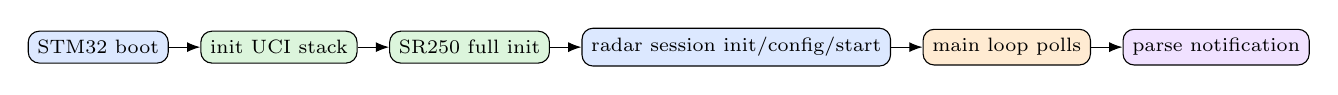
\begin{tikzpicture}[font=\scriptsize,node distance=0.35cm,>=Latex]
\node[draw,rounded corners,fill=bluepale] (boot) {STM32 boot};
\node[draw,rounded corners,fill=greenpale,right=0.4cm of boot] (init) {init UCI stack};
\node[draw,rounded corners,fill=greenpale,right=0.4cm of init] (sr) {SR250 full init};
\node[draw,rounded corners,fill=bluepale,right=0.4cm of sr] (sess) {radar session init/config/start};
\node[draw,rounded corners,fill=orangepale,right=0.4cm of sess] (loop) {main loop polls};
\node[draw,rounded corners,fill=purplepale,right=0.4cm of loop] (ntf) {parse notification};
\draw[->] (boot) -- (init);
\draw[->] (init) -- (sr);
\draw[->] (sr) -- (sess);
\draw[->] (sess) -- (loop);
\draw[->] (loop) -- (ntf);
\end{tikzpicture}

\medskip
\begin{tcolorbox}[summarybox={Runtime Story}]
\begin{enumerate}
  \item Board peripherals come up.
  \item UCI transport/core are initialized.
  \item SR250 is reset and prepared.
  \item A radar session is created.
  \item Standard and vendor radar parameters are written.
  \item Session is started.
  \item Forever loop:
  \begin{itemize}
    \item poll UCI,
    \item decode notifications,
    \item print metadata,
    \item send raw CIR packets over UDP.
  \end{itemize}
\end{enumerate}
\end{tcolorbox}

% ============================================================
\section*{5.\ What main.c Does}
% ============================================================

\texttt{main.c:175--178} initializes the UCI stack:
\[
\texttt{uci\_transport\_init()}
\rightarrow
\texttt{uci\_core\_init()}
\rightarrow
\texttt{uci\_core\_register\_ntf\_callback(...)}
\]

\texttt{main.c:183--194} builds an \texttt{uci\_sr250\_init\_config\_t} with:
\begin{itemize}
  \item RX antenna definitions,
  \item TX antenna definitions,
  \item RX antenna pair definitions,
  \item channel 9.
\end{itemize}

\texttt{main.c:203--255} creates and configures the radar session.

\texttt{main.c:275} repeatedly calls \texttt{uci\_core\_process()}.
That is the heartbeat of the whole communication stack.

\begin{tcolorbox}[warnbox={Very Important}]
The code after the \texttt{while(1)} loop never executes in normal operation.
So the later calls to:
\begin{itemize}
  \item \texttt{uci\_radar\_stop()}
  \item \texttt{uci\_radar\_deinit()}
\end{itemize}
are effectively dead code unless you re-enable the commented break logic.
\end{tcolorbox}

% ============================================================
\section*{6.\ Current Radar Configuration}
% ============================================================

\begin{tabular}{@{}p{2.5cm}p{4.8cm}@{}}
\toprule
Field & Current value in \texttt{main.c} \\
\midrule
mode & \texttt{UCI\_RADAR\_MODE\_MEDIUM\_DISTANCE} \\
channel & 9 \\
preamble & 26 \\
CIR samples & 128 \\
RFRI interval & 96 ms \\
slots per RR & 4 \\
RX antennas & RXC=1, RXB=2, RXA=0 \\
TX antenna & 1 \\
presence mode & \texttt{0x00} \\
max measurements & 0 (unlimited) \\
\bottomrule
\end{tabular}

\begin{tcolorbox}[warnbox={Reality Check: Intended vs Actual}]
The comment in \texttt{main.c} says:
\begin{center}
\texttt{Start a radar session with presence detection + AoA}
\end{center}
but the actual configuration does \textbf{not} fully match that intent:
\begin{itemize}
  \item \texttt{presence\_det.mode = 0x00} means the presence TLV is not sent at all.
  \item \texttt{uci\_radar\_configure()} only sends presence config if mode is nonzero.
  \item the 50 ms OCPD check is only enforced if presence mode bit0 is enabled.
\end{itemize}
So as written, this firmware looks much more like a \textbf{CIR streaming setup with antennas prepared for AoA}, not a fully enabled presence-detection configuration.
\end{tcolorbox}

\textbf{Another subtle point:}
\texttt{ranging\_interval\_ms = 96} conflicts with the nearby comment saying 50 ms is required for OCPD. That mismatch currently slips through only because presence mode is disabled.

% ============================================================
\section*{7.\ SR250 Full Initialization}
% ============================================================

\texttt{uci\_sr250\_full\_init()} in \texttt{uci\_sr250.c:348+} does the chip bring-up sequence.

\begin{tcolorbox}[intubox={Initialization Sequence}]
\begin{enumerate}
  \item Hardware reset line toggle.
  \item Wait for device status notification = READY.
  \item Send software device reset command.
  \item Wait for READY again.
  \item Send NXP device init command.
  \item Wait for READY again.
  \item Program RX antenna definitions.
  \item Program TX antenna definitions.
  \item Program RX antenna pairs.
  \item Read device info.
\end{enumerate}
\end{tcolorbox}

\textbf{Plain English:}
the code makes sure the chip is alive, then teaches it what the board wiring looks like, then asks for confirmation that the chip can talk UCI correctly.

\begin{tcolorbox}[analogybox={Analogy --- Introducing A New Robot To A Lab}]
Imagine a robot arrives in a lab.
You do not immediately give it a task.
First you:
\begin{itemize}
  \item power cycle it,
  \item wait until it says ``I am ready'',
  \item load its hardware map,
  \item then assign work.
\end{itemize}
That is exactly what \texttt{uci\_sr250\_full\_init()} is doing.
\end{tcolorbox}

\begin{tcolorbox}[warnbox={Important Mismatch}]
\texttt{main.c} sets \texttt{run\_chip\_calibration = true}, but in \texttt{uci\_sr250.c} the calibration block is commented out.
So calibration is \textbf{requested by configuration but not actually executed}.
\end{tcolorbox}

% ============================================================
\section*{8.\ Antenna Database}
% ============================================================

The board-specific arrays at the top of \texttt{main.c} define how logical antenna IDs map to physical ports:
\begin{itemize}
  \item RX antenna IDs \texttt{0x01..0x04}
  \item TX antenna IDs \texttt{0x01..0x02}
  \item RX pairs that tell the chip which antennas form valid combinations
\end{itemize}

\textbf{Why this matters:}
the SR250 cannot infer your PCB wiring. You must explicitly tell it:
\begin{itemize}
  \item which ID corresponds to RXC/RXB/RXA,
  \item which TX port is TRA1/TRA2,
  \item and which pairings are valid.
\end{itemize}

\begin{tcolorbox}[newbox={Host View vs Chip View}]
\begin{tabular}{@{}p{2.6cm}p{4.7cm}@{}}
\textbf{Host view} & ``Use antenna ID 0x02'' \\
\textbf{Chip needs} & ``0x02 means RXB on this specific board'' \\
\end{tabular}
\end{tcolorbox}

% ============================================================
\section*{9.\ Layered Stack}
% ============================================================

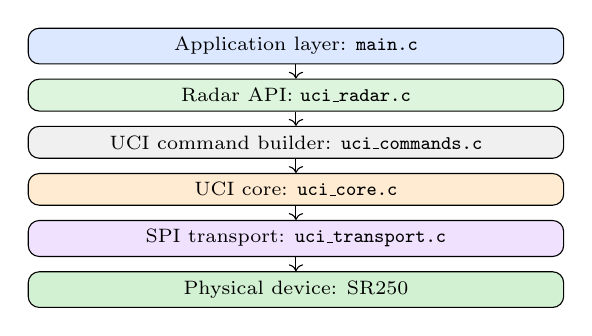
\begin{tikzpicture}[font=\scriptsize,node distance=0.18cm]
\node[draw,rounded corners,fill=bluepale,minimum width=6.8cm] (a) {Application layer: \texttt{main.c}};
\node[draw,rounded corners,fill=greenpale,below=of a,minimum width=6.8cm] (b) {Radar API: \texttt{uci\_radar.c}};
\node[draw,rounded corners,fill=graypale,below=of b,minimum width=6.8cm] (c) {UCI command builder: \texttt{uci\_commands.c}};
\node[draw,rounded corners,fill=orangepale,below=of c,minimum width=6.8cm] (d) {UCI core: \texttt{uci\_core.c}};
\node[draw,rounded corners,fill=purplepale,below=of d,minimum width=6.8cm] (e) {SPI transport: \texttt{uci\_transport.c}};
\node[draw,rounded corners,fill=greenlt,below=of e,minimum width=6.8cm] (f) {Physical device: SR250};
\draw[->] (a) -- (b);
\draw[->] (b) -- (c);
\draw[->] (c) -- (d);
\draw[->] (d) -- (e);
\draw[->] (e) -- (f);
\end{tikzpicture}

\textbf{Interpretation:}
\begin{itemize}
  \item Upper layers think in terms of sessions, antennas, and presence detection.
  \item Lower layers think in bytes, headers, payload lengths, and SPI timing.
\end{itemize}

% ============================================================
\section*{10.\ UCI Command Flow}
% ============================================================

\texttt{uci\_radar\_configure()} is the most important configuration function.
Its flow is:

\begin{enumerate}
  \item validate semantic constraints,
  \item build standard app-config TLVs,
  \item send them with \texttt{uci\_cmd\_session\_set\_app\_config()},
  \item build vendor radar TLVs,
  \item send them with \texttt{uci\_sr250\_set\_vendor\_app\_config()}.
\end{enumerate}

\begin{tcolorbox}[formulabox={Mental Model}]
\[
\text{high-level struct}
\rightarrow
\text{TLVs}
\rightarrow
\text{UCI packet}
\rightarrow
\text{SPI transaction}
\]
\end{tcolorbox}

\textbf{Why there are two config phases:}
\begin{itemize}
  \item \textbf{standard app config} uses FiRa/UCI-style tags such as channel and preamble,
  \item \textbf{vendor app config} uses NXP radar-specific tags such as radar mode, CIR samples, RX gain, RFRI, presence detection configuration.
\end{itemize}

% ============================================================
\section*{11.\ Validation Logic}
% ============================================================

\texttt{uci\_radar\_configure()} performs two important checks before sending anything:

\begin{enumerate}
  \item If AoA is requested (\texttt{presence\_det.mode \& 0x02}), it requires at least two nonzero RX antenna IDs.
  \item If presence detection is enabled (\texttt{mode bit0}) and RFRI is used, then \texttt{ranging\_interval\_ms} must equal 50.
\end{enumerate}

\begin{tcolorbox}[analogybox={Analogy --- Ticket Checker}]
Before the code lets the session board the train, it checks:
\begin{itemize}
  \item ``If you want angle, did you bring enough antennas?''
  \item ``If you want OCPD presence mode, did you choose the right timing?''
\end{itemize}
If not, it rejects the request immediately.
\end{tcolorbox}

% ============================================================
\section*{12.\ TLVs Written For Radar}
% ============================================================

\begin{tabular}{@{}p{2.2cm}p{5.0cm}@{}}
\toprule
Tag & Meaning \\
\midrule
\texttt{CHANNEL\_NUMBER} & UWB channel \\
\texttt{PREAMBLE\_CODE\_INDEX} & preamble selection \\
\texttt{ANTENNAS\_CONFIG\_RX} & radar RX mode + selected RX IDs \\
\texttt{ANTENNAS\_CONFIG\_TX} & selected TX antenna \\
\texttt{RADAR\_MODE} & medium/close/far/etc. \\
\texttt{RADAR\_SINGLE\_FRAME\_NTF} & notification policy \\
\texttt{RADAR\_RFRI} & frame timing tuple \\
\texttt{RADAR\_CIR\_NUM\_SAMPLES} & number of CIR samples \\
\texttt{RADAR\_RX\_GAIN} & AGC/manual gain fields \\
\texttt{RADAR\_CIR\_START\_OFFSET} & where CIR acquisition starts \\
\texttt{RADAR\_PERFORMANCE} & performance flags \\
\texttt{RADAR\_DRIFT\_COMPENSATION} & compensation coefficient \\
\texttt{RADAR\_PRESENCE\_DET\_CFG} & presence window and thresholds \\
\bottomrule
\end{tabular}

\textbf{Interpretation:}
this firmware mostly tells the chip:
\begin{itemize}
  \item \emph{where} to listen,
  \item \emph{how often} to measure,
  \item \emph{what outputs} to produce,
  \item and \emph{which antennas} define the geometry.
\end{itemize}

% ============================================================
\section*{13.\ Header And Packet Basics}
% ============================================================

UCI packets have a 4-byte header:
\begin{itemize}
  \item message type (CMD, RSP, NTF, DATA),
  \item packet boundary flag,
  \item group ID,
  \item opcode ID,
  \item payload length.
\end{itemize}

\begin{tcolorbox}[newbox={UCI Header}]
\begin{tabular}{@{}ll@{}}
Byte 0 & MT[7:5], PBF[4], GID[3:0] \\
Byte 1 & EXT bit and OID \\
Byte 2 & RFU or payload length LSB \\
Byte 3 & payload length or MSB depending on EXT \\
\end{tabular}
\end{tcolorbox}

\texttt{uci\_build\_header()} creates this layout.
\texttt{uci\_parse\_header()} reverses it.

\textbf{Extended-length support:}
if payload length exceeds 255, the code sets the NXP EXT bit and uses a 16-bit length field.

% ============================================================
\section*{14.\ SPI Transport}
% ============================================================

The transport layer is not plain SPI payload transfer. It adds a direction byte:
\begin{itemize}
  \item \texttt{0x00} for write,
  \item \texttt{0xFF} for read.
\end{itemize}

\begin{tcolorbox}[intubox={Two-Phase Read}]
\textbf{Phase 1:} read only the UCI header.\\
\textbf{Phase 2:} now that length is known, read exactly that many payload bytes.
\end{tcolorbox}

\textbf{Why this is necessary:}
SPI itself does not tell you packet size. The host must first ask for the header, decode the length, then ask for the remaining bytes.

\begin{tcolorbox}[analogybox={Analogy --- Reading A Mailing Label First}]
Before opening a package, you first read the label to know:
\begin{itemize}
  \item who sent it,
  \item what kind of package it is,
  \item and how big it is.
\end{itemize}
The transport layer does the same thing with the UCI header.
\end{tcolorbox}

The code also inserts timing delays:
\begin{itemize}
  \item post-write delay,
  \item pre-read delay,
  \item inter-phase read delay.
\end{itemize}
Those are there to respect the SR250 timing behavior.

% ============================================================
\section*{15.\ Core Engine Behavior}
% ============================================================

\texttt{uci\_core\_send\_command()} does five jobs:
\begin{enumerate}
  \item build a command packet,
  \item fragment it if too large,
  \item send it through transport,
  \item poll until the matching response arrives,
  \item copy the response payload back to the caller.
\end{enumerate}

\texttt{uci\_core\_process()} does the receive-side work:
\begin{enumerate}
  \item if the SR250 INT line says data is ready, read one packet,
  \item parse the header,
  \item reassemble fragments if needed,
  \item dispatch the packet as response or notification.
\end{enumerate}

\begin{tcolorbox}[summarybox={Single Outstanding Command Window}]
This implementation assumes only one command is waiting for a response at a time.
That matches the intended UCI style here: send command, wait, continue.
\end{tcolorbox}

% ============================================================
\section*{16.\ Response vs Notification}
% ============================================================

\textbf{Response:}
comes back because the host explicitly asked something.

\textbf{Notification:}
arrives asynchronously because the chip wants to report a state change or radar result.

\begin{tcolorbox}[newbox={Examples}]
\begin{tabular}{@{}p{2cm}p{5.1cm}@{}}
\textbf{Response} & ``Yes, your session start command succeeded.'' \\
\textbf{Notification} & ``A new CIR block is available.'' \\
\end{tabular}
\end{tcolorbox}

\texttt{uci\_dispatch\_packet()} in \texttt{uci\_core.c} separates these cases.

\textbf{Retry behavior:}
if the first byte of a response or notification payload is \texttt{UCI\_STATUS\_MESSAGE\_RETRY}, the code retransmits the last command.

% ============================================================
\section*{17.\ Fragmentation}
% ============================================================

Large UCI packets may arrive in segments.
\texttt{uci\_process\_raw\_packet()} uses the packet-boundary flag (PBF):
\begin{itemize}
  \item \texttt{SEGMENT}: append payload to reassembly buffer,
  \item \texttt{COMPLETE}: either dispatch directly or finish a multi-part packet.
\end{itemize}

\textbf{Why it matters for radar:}
CIR notifications can be large, so the stack must handle data that may not fit in a single UCI payload.

% ============================================================
\section*{18.\ Notification Handler In main.c}
% ============================================================

\texttt{app\_uci\_notification\_handler()} is the application-level decoder.

It checks:
\begin{itemize}
  \item radar notifications,
  \item device status notifications,
  \item session status notifications.
\end{itemize}

\textbf{Radar path:}
\begin{enumerate}
  \item identify radar data type via \texttt{uci\_radar\_get\_ntf\_type()},
  \item switch on the type,
  \item call the matching parser,
  \item print or forward the result.
\end{enumerate}

\begin{tcolorbox}[intubox={Current App Behavior}]
\begin{itemize}
  \item CIR notification:
  parse metadata, then forward the \emph{raw payload} over UDP port 20000.
  \item Presence notification:
  print target distance and angle.
  \item Antenna isolation notification:
  print TX-to-RX isolation in dB.
\end{itemize}
\end{tcolorbox}

% ============================================================
\section*{19.\ CIR Notification Layout}
% ============================================================

\texttt{uci\_radar\_parse\_cir\_ntf()} expects:

\begin{tcolorbox}[newbox={RADAR\_RX\_NTF for CIR}]
\begin{tabular}{@{}ll@{}}
Common header & \texttt{[session\_handle:4][status:1][type:1]} \\
Block header & \texttt{[num\_samples:2][taps\_per\_sample:1][rfu:1]} \\
Metadata & first 32 bytes = TAP[0] to TAP[7] \\
Actual CIR & remaining bytes = TAP[8+] \\
\end{tabular}
\end{tcolorbox}

\textbf{What the parser returns:}
\begin{itemize}
  \item a filled \texttt{uci\_radar\_cir\_metadata\_t},
  \item a pointer to the start of the actual CIR data,
  \item and a computed number of CIR taps.
\end{itemize}

\textbf{Important design choice:}
\texttt{cir\_data\_out} points \emph{into the original payload}. The parser does not copy the CIR array.

% ============================================================
\section*{20.\ CIR Metadata Fields}
% ============================================================

The parser extracts:
\begin{itemize}
  \item counters and timestamps,
  \item tap resolution bits,
  \item gain indices,
  \item TX/RX antenna IDs,
  \item RX path,
  \item radar mode flags,
  \item pulse-shape and pulse-count info,
  \item CIR start offset.
\end{itemize}

\textbf{Why this metadata matters:}
without it, raw taps are just numbers. Metadata tells you which antenna, which timing, and which acquisition mode produced those numbers.

\begin{tcolorbox}[analogybox={Analogy --- A Photo Needs EXIF Metadata}]
A JPEG without EXIF is just pixels.
The metadata tells you:
\begin{itemize}
  \item which camera,
  \item what exposure,
  \item when it was taken.
\end{itemize}
CIR metadata plays the same role for radar samples.
\end{tcolorbox}

% ============================================================
\section*{21.\ CIR Tap Extraction}
% ============================================================

\texttt{uci\_radar\_get\_cir\_tap()} assumes:
\begin{itemize}
  \item 3 bytes per tap,
  \item 16-bit signed real part from bytes 0--1,
  \item 8-bit signed imaginary part from byte 2, sign-extended to 16 bits.
\end{itemize}

\begin{tcolorbox}[formulabox={Tap Interpretation}]
\[
\text{offset} = 3 \cdot \text{tap\_index}
\]
\[
\text{real} = \text{int16}(\text{byte}_0,\text{byte}_1)
\qquad
\text{imag} = \text{sign-extended int8}(\text{byte}_2)
\]
\end{tcolorbox}

\begin{tcolorbox}[warnbox={Implementation Assumption}]
The helper only decodes the default 3-byte format.
The commented code suggests 24-bit or 32-bit tap formats may exist, but they are not implemented here.
\end{tcolorbox}

% ============================================================
\section*{22.\ Presence Notification Layout}
% ============================================================

\texttt{uci\_radar\_parse\_presence\_ntf()} expects after the common 6-byte header:
\begin{itemize}
  \item \texttt{presence\_detected},
  \item \texttt{presence\_mode},
  \item \texttt{num\_detections},
  \item then per target:
  \begin{itemize}
    \item distance in cm,
    \item signed angle in degrees,
    \item 4-byte float SNR trigger,
    \item SNR-valid flag.
  \end{itemize}
\end{itemize}

\textbf{Plain English:}
the chip is doing the hard sensing internally and sending back a short report card:
\begin{center}
``I saw this many targets; here are their distances and angles.''
\end{center}

% ============================================================
\section*{23.\ Antenna Isolation Notification}
% ============================================================

This is the simplest radar notification:
\[
\texttt{[session\_handle][status][type][tx\_id][rx\_id][isolation\_db]}
\]

\textbf{Meaning:}
it measures how much TX leaks into RX directly.
Large leakage can hurt radar quality because it can bury weak reflections.

% ============================================================
\section*{24.\ Plain-English Flow Of A CIR Packet}
% ============================================================

\begin{enumerate}
  \item SR250 finishes a measurement.
  \item It raises its interrupt line.
  \item STM32 main loop calls \texttt{uci\_core\_process()}.
  \item Transport reads the UCI header, then payload.
  \item Core decides this is a notification.
  \item App callback sees it is \texttt{RADAR\_RX\_NTF}.
  \item App asks: ``Which radar data type is this?''
  \item For CIR type, parser extracts metadata and locates raw taps.
  \item The entire raw payload is sent over UDP port 20000.
  \item A short summary is printed on UART.
\end{enumerate}

\begin{tcolorbox}[analogybox={Analogy --- Warehouse Receiving}]
\begin{itemize}
  \item Doorbell rings: interrupt line.
  \item Clerk checks label: UCI header.
  \item Package goes to correct department: response vs notification.
  \item Radar desk opens the box and sorts:
  \begin{itemize}
    \item metadata sheet,
    \item actual signal samples.
  \end{itemize}
  \item Shipping desk forwards the raw box over UDP.
\end{itemize}
\end{tcolorbox}

% ============================================================
\section*{25.\ Function-by-Function Reference}
% ============================================================

\begin{tabular}{@{}p{2.7cm}p{4.3cm}@{}}
\toprule
Function & What it means \\
\midrule
\texttt{uci\_transport\_init} & enable microsecond delay support \\
\texttt{uci\_core\_init} & reset internal UCI state machine \\
\texttt{uci\_sr250\_full\_init} & bring SR250 to usable state \\
\texttt{uci\_radar\_session\_init} & create radar session handle \\
\texttt{uci\_radar\_configure} & convert struct into standard + vendor TLVs \\
\texttt{uci\_radar\_start} & tell session to begin measuring \\
\texttt{uci\_core\_process} & poll and process one incoming packet \\
\texttt{uci\_radar\_get\_ntf\_type} & inspect byte 5 of radar payload \\
\texttt{uci\_radar\_parse\_cir\_ntf} & decode CIR block header and metadata \\
\texttt{uci\_radar\_parse\_presence\_ntf} & decode presence report \\
\texttt{uci\_radar\_parse\_ant\_isolation\_ntf} & decode isolation test report \\
\bottomrule
\end{tabular}

% ============================================================
\section*{26.\ What The MCU Computes vs What The Chip Computes}
% ============================================================

\begin{tcolorbox}[newbox={Responsibility Split}]
\begin{tabular}{@{}p{2.5cm}p{4.6cm}@{}}
\textbf{STM32 computes} & packet formatting, TLVs, header parsing, byte decoding, forwarding, printing \\
\textbf{SR250 computes} & UWB radar measurement, CIR generation, presence decision, angle-related result generation \\
\end{tabular}
\end{tcolorbox}

\textbf{This is one of the most important conceptual points in the whole project.}
If you want to change detection quality, antenna geometry, or radar mode, you mostly change \textbf{configuration}. If you want to change how bytes move around or how logs look, you change the STM32 firmware.

% ============================================================
\section*{27.\ Important Caveats In The Current Code}
% ============================================================

\begin{tcolorbox}[warnbox={Caveat 1 --- Presence Not Actually Enabled}]
\texttt{presence\_det.mode = 0x00} means presence configuration is skipped.
So the code comments overstate what is currently enabled.
\end{tcolorbox}

\begin{tcolorbox}[warnbox={Caveat 2 --- Calibration Flag Not Used}]
\texttt{run\_chip\_calibration = true} is set in \texttt{main.c}, but the actual calibration call is commented out in \texttt{uci\_sr250\_full\_init()}.
\end{tcolorbox}

\begin{tcolorbox}[warnbox={Caveat 3 --- Stop/Deinit Unreachable}]
Because the loop is infinite, shutdown code is not reached unless you restore a break condition.
\end{tcolorbox}

\begin{tcolorbox}[warnbox={Caveat 4 --- Possible TX Antenna Struct Packing Typo}]
In \texttt{uci\_sr250\_set\_tx\_antenna\_defs()}, byte \texttt{off+5} is filled with \texttt{gpio\_mask\_msb} instead of \texttt{gpio\_state\_msb}. This is harmless right now because the configured values are all zero, but it is worth noticing.
\end{tcolorbox}

\begin{tcolorbox}[warnbox={Caveat 5 --- CIR Helper Assumes One Format}]
\texttt{uci\_radar\_get\_cir\_tap()} only handles the default 3-byte/tap interpretation. If the SR250 changes resolution mode, this helper will not decode taps correctly.
\end{tcolorbox}

% ============================================================
\section*{28.\ Mental Model For Debugging}
% ============================================================

When something fails, ask the question in layers:
\begin{enumerate}
  \item Is the board and SPI transport alive?
  \item Is the UCI core receiving valid headers?
  \item Did the SR250 reach READY state?
  \item Did session init/config/start return \texttt{UCI\_STATUS\_OK}?
  \item Is the main loop polling \texttt{uci\_core\_process()} often enough?
  \item Is the notification type what you think it is?
  \item Are the comments lying, or are the actual field values correct?
\end{enumerate}

\begin{tcolorbox}[summarybox={Best Debugging Principle}]
In this codebase, many ``radar problems'' are really one of three things:
\begin{itemize}
  \item configuration mismatch,
  \item packet parsing mismatch,
  \item or comments no longer matching the current code.
\end{itemize}
\end{tcolorbox}

% ============================================================
\section*{29.\ If You Want True Presence + AoA}
% ============================================================

\textbf{Based on the current implementation logic, the configuration would need at least:}
\begin{itemize}
  \item \texttt{presence\_det.mode} with bit0 enabled, and probably bit1 as well,
  \item two nonzero RX antennas,
  \item RFRI interval of 50 ms if you want the OCPD-constrained mode enforced by \texttt{uci\_radar\_configure()}.
\end{itemize}

\textbf{Conceptually:}
you already have the plumbing in place.
The missing piece is not a new parser; it is making the configuration values match the intended mode.

% ============================================================
\section*{30.\ Compact Summary}
% ============================================================

\begin{tcolorbox}[summarybox={SR250 Radar Firmware --- Quick Reference}]
\textbf{What the code does:}
STM32 configures and polls an SR250 radar chip using UCI over SPI.
The chip does the sensing; the STM32 moves bytes and interprets reports.

\smallskip
\textbf{Main runtime loop:}
\[
\texttt{uci\_core\_process()}
\rightarrow
\texttt{notification callback}
\rightarrow
\texttt{parse}
\rightarrow
\texttt{print / UDP send}
\]

\textbf{Most important files:}
\begin{itemize}
  \item \texttt{main.c}: boot, session config, notification handler
  \item \texttt{uci\_radar.c}: radar TLVs and radar packet parsing
  \item \texttt{uci\_core.c}: send/wait/reassemble/dispatch engine
  \item \texttt{uci\_transport.c}: SPI wire protocol
  \item \texttt{uci\_sr250.c}: SR250-specific startup and antenna database programming
\end{itemize}

\textbf{Most important conceptual lesson:}
\textbf{This firmware is a control-and-parse layer, not the radar algorithm itself.}

\smallskip
\textbf{Biggest current mismatches:}
\begin{itemize}
  \item comments say presence + AoA, but presence mode is disabled,
  \item calibration flag is set, but calibration call is commented out,
  \item stop/deinit code is unreachable under the infinite loop.
\end{itemize}
\end{tcolorbox}

\end{multicols*}
\end{document}
